\documentclass[12pt]{article}
\renewcommand{\thesubsection}{\thesection.\alph{subsection}}
\usepackage{amsmath}  % flere
\usepackage[utf8]{inputenc} % æøå
\usepackage[T1]{fontenc} % mere æøå
\usepackage[danish]{babel} % orddeling
\usepackage{graphicx}
\usepackage{amsfonts}
\usepackage{hyperref}
\usepackage[indent = 0pt]{parskip}

\title{\textbf{Projekt 4: PageRank}\\
02525 - Gruppe: Januar 8}
\author{Kaj: s224371\\  Sami: s224386\\ Ibrahim: s224403\\ August: s224367}
\date{ \textbf{18. januar 2023} }

\begin{document}

\maketitle
\tableofcontents
\newpage

\section{PageRank}
Formålet med PageRank algoritmen er at estimere den relative relevans af hjemmesider. Det forestilles en person som tilfældigt klikker på et hyperlink på den nuværende hjemmeside for at komme videre til en ny hjemmeside. Denne person starter på en tilfældig hjemmeside. En hjemmesides PageRank er så chancen for at finde denne person på en hjemmeside, til et vilkårligt tidspunkt. Resultatet kan så fortolkes som at en større PageRank svarer til en større relevans.

\subsection*{Dæmpningsfaktor}
\begin{figure}[!h]
    \centering
    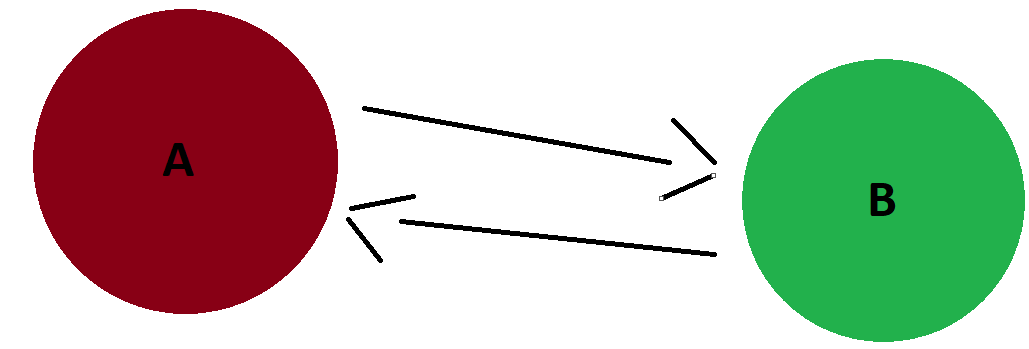
\includegraphics[width = \linewidth]{Billeder/damping_fac.png}
    \caption{Illustration af det beskrevne nedenunder. Udarbejdet af os.}
    \label{fig:my_label}
\end{figure}

Når man går ind på en hjemmeside vil der oftest være såkaldte hyperlinks der tager brugeren til en anden hjemmeside. Lad os betragte en situation hvor en hjemmeside A kun linker til en hjemmeside B og hjemmeside B kun linker til hjemmeside A. Når dette er tilfældet, og man kører vores algoritme vil man jo netop sidde fast ved disse to hjemmesider under hele forløbet, og således vil det være vanskeligt at bestemme en "ordentlig"  PageRank. For at undgå dette har vi en såkaldt dæmpningsfaktor, $d$ (eng.: damping factor). Formålet med denne er at give en mulighed for at dæmpe algortimen ved algoritmens næste skridt. Dette skal forstås således: Enten udvælges et tilfældigt hyperlink på den nuværende hjemmeside eller udvælges en tilfældig hjemmeside i vores sæt af hjemmesider ($W$). En almindelig værdi for $d$ er 0.85, dvs. 85\% sandsynlighed for at udvælge et tilfældigt hyperlink som hjemmeside $P_i$ linker til og $1 - d = 0.15$ dvs. 15\% sandsynlighed for at udvælge en tilfældig hjemmeside i sættet $W$ (nuværende hjemmeside inkluderet).

\subsection*{Tilgange til projektet}

\textbf{Random Surfer Model}


For at videreuddybe konceptet beskrevet foroven: Vi har et sæt af hjemmesider, $W$, hvorledes der er $N$-antal hjemmesider. For hver (men ikke nødvendigvis alle) hjemmeside $P_i$ er der et vis antal hyperlinks der fører videre til en anden hjemmeside. Dette er det grundlæggende for at kunne bestemme det såkaldte PageRank. En metode til denne algoritme er \emph{Random Surfer Model}, hvor der indledningsvist udvælges en tilfældig hjemmeside i sættet $W$, dvs. hver hjemmeside har sandsynligheden $\frac{1}{N}$ for at bliver udvalgt i starten. Efterfølgende vil modellen således udvælge et tilfældigt hyperlink på den nuværende hjemmeside $P_i$, som fører til en anden hjemmeside i sættet $W$. Hvert besøg hos hjemmesiden bliver talt og gemt. Hvis modellen har kørt $n$-gange og en hjemmeside $P_k$ er blevet besøgt $N_k$ gange vil $\frac{N_k}{n}$ således være sandsynligheden for at ankomme på hjemmesiden tilfældigt. Og i teorien hvis dette kører nok gange (hvis $n \rightarrow \infty$, eller hvis det måles i tid $t \rightarrow \infty$) vil dette netop være hjemmesiden $P_k$'s såkaldte PageRank. Dæmpningsfaktoren kommer i spil netop der hvor modellen udvælger et tilfældigt hyperlink på nuværende hjemmeside $P_i$, som beskrevet i afsnittet "Dæmnpningsfaktor". Dette er jo som sagt for at bekæmpe instanser hvor en hjemmeside er et såkaldt "sink" (ingen hyperlinks) eller hvis to hjemmesider kun fører til hinanden.


\textbf{Rekursive model}

Den reukursive formel er givet ved
\begin{equation} \label{udgangspunkt}
    PR(p_i)_{n+1}=\frac{1-d}N+d\sum_{p_j\in Inbound(p_i)}\frac{PR(p_j)_n}{\left|Outbound(p_j)\right|}
\end{equation}

Her er $PR(p_i)$ PageRank for $p_i$. $Inbound(p_i)$ er det sæt af websites som linker til $p_i$ og $Outbound(p_j)$ er det sæt af websites som linker væk fra $p_j$.

Det første led i \eqref{udgangspunkt} tager hensyn til situationen hvor der linkes til en ny tilfældig website pga. dæmpningsfaktoren. Dette er udtrykt matematisk ved at der er lige stor sandsynlighed for at lande på alle, så chancen er $\frac1N$, som så bliver vægtet med $1-d$, da $1-d$ er chancen for at der skal bevæges til et tilfældigt website.

Det andet led i \eqref{udgangspunkt} tager hensyn til situationen hvor der bliver bevæget sig hen til websitet fra en anden website. Denne kommer fra at summere chancen for at komme til $p_i$ ved for alle de websites $p_j$ som linker til $p_i$. Chancen for at komme til $p_i$ fra et website $p_j$, som linker til $p_i$ er
\begin{equation*}
    \frac{d\cdot PR(p_j)}{\left|Outbound(p_j)\right|}
\end{equation*}
Dette er i virkeligheden chancen for at der tilfældigvis landes på $p_i$ ud fra alle de andre websites som $p_j$ linker til ved $\frac1{\left|Outbound(p_j)\right|}$. Denne chance er så vægtet med $PR(p_j)$, da PageRank af $p_j$ angiver chancen for at befinde sig på $p_j$, og det skal være tilfældet, da man ellers ikke kan bevæge sig fra $p_j$ til $p_i$. Der bliver også vægtet med dæmpningsfaktoren, da det også skal være tilfældet at der bliver bevæget sig fra $p_j$ til et website den forbindet til, og ikke bare til en tilfældig website ud af alle websites med en ligelig sandsynlighedsfordeling.



\textbf{Matrixformulation}


\subsection*{title}

\subsection*{Beskrivelse af programmet}




\subsection*{Illustrationer og eksempler}
\newpage

\section{Programmerings opgaver}



\subsection*{Programmering opgaver 1.}



\subsection*{Programmering opgaver 2.}



\subsection*{Programmering opgaver 3.}


\subsection*{Tids overvejelser}
\subsubsection*{Hvordan beregnes tiden af en funktion i Python}
For at få konkrete værdier for hvor lang tid det tager metoderne at beregne PageRank værdierne, så brugte vi \emph{time} modulet indbygget i Python. Her kan der bruges \texttt{time.time()} til at gemme en start-tid før funktionen er startet og en tid når den er stoppet. Den totale tid det tager beregnes så ved at trække start-tiden fra stop-tiden.

\subsubsection*{Analyse af data}
\begin{table}[!h]
    \centering
    \begin{tabular}{c|l|l|l|l}
        Antal hjemmesider & Random Surfer & Recursive & Limit & Eigenvectors \\
        \hline
        $N = 10$       & 1.8134 s   & 0.0000 s   & 0.0000 s   & 0.0010 s   \\
        $N = 75$       & 3.4769 s   & 0.0110 s   & 0.0020 s   & 0.0028   \\
        $N = 250$      & 7.6943 s   & 0.0860 s   & 0.0090 s   & 0.0699
    \end{tabular}
    \caption{En tabel over metodernes tidsforbrug afhængigt at $n$, antallet af webpages i simulationen. Når der står "0.0000" så betyder det ikke faktisk 0, men skyldes numeriske fejl fra python fordi tallet er så lille. Her refererer "Random Surfer" til Random surfer modellen med en dæmpningsfaktor, "Recursive" er den rekursive model, "Limit" er hvor der anvendes at $A$ er en \textit{Markov matrix} med positive værdier og "Eigenvectors er hvor der findes den korrekte egenvektor og den skaleres tilpasseligt. Naturligvis er dæmpningsfaktoren $d$ ens for alle modellerne som er $d = 0.85$.}
    \label{tidsFigur}
\end{table}

\begin{figure}
    \centering
    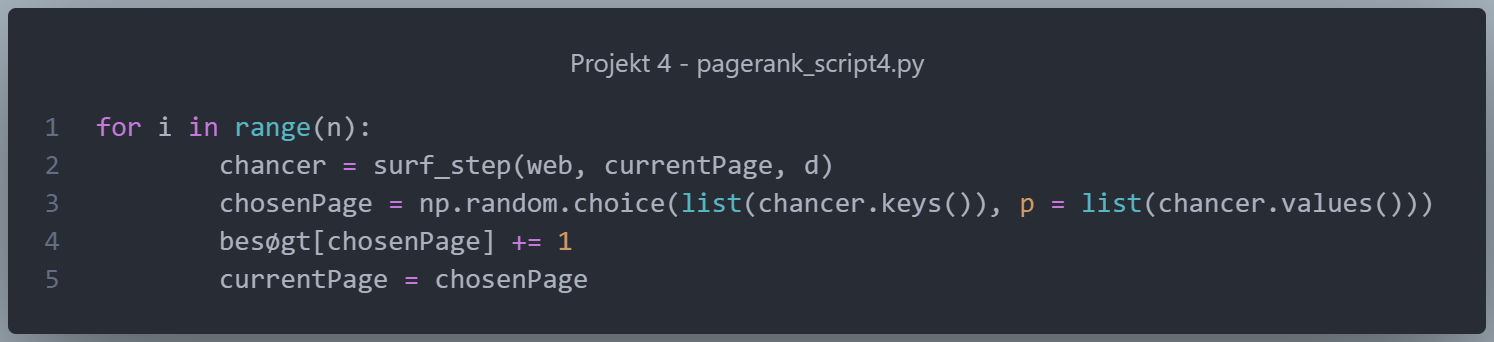
\includegraphics[width = \linewidth]{Kode1.png}
    \caption{Del af kode fra \texttt{random\_surfer} funktionen}
\end{figure}


På Tabel~\ref{tidsFigur}, kan det ses at Random Surfer modellen er den klart mest langsomme model som der er. Dette giver også mening siden at der for hver iteration af algoritmen skal køres \texttt{surf\_step} funktionen, som beregner sandsynlighedsfordelingen. En hurtig måde der kunne skæres ned på tiden brugt i denne funktion, vil være ved at gemme resultatet af \texttt{surf\_step} og så genbruge det, så det ikke skal beregnes hver gang igen.

Det kan ses ved at kigge på alle resultaterne at Limit-metoden er klart den hurtigste. Denne I dette tilfælde har vi dog ganget matricen med sig selv 20 gange. Denne værdi kan forøges så meget som man vil, på bekostningen af det så vil tage længere tid, men resultatet vil blive mere præcist.

Den rekursive model kan også tilpasses så den tager mindre tid, ved at ændre på \texttt{stopvalue} eller \texttt{max\_iterations}.

Egenværdi metoden virker som den som generelt er bedst, da den finder den matematiske korrekte løsning og tager meget kort tid



\newpage


\section{Løsninger til teoretiske problemer:}


\subsection*{Problem 1.}

Ligningen (2.3) viser, at x er lig med en kombination af to ting: $\frac{(1-d)}{N}e$ og $d\cdot L\cdot x$. $e$ er en vektor bestående af kun 1'ere, $E_N$ er en matrix bestående af kun 1'ere.
Da $L$ er en kendt matrix, og $d$ er en kendt konstant og $N$ er en kendt heltal, kan vi erstatte e og $E_N$ i ligningen (2.3) for at få :
$$x = \frac{(1-d)}{N}E_N + d\cdot L\cdot x$$
Vi kan derefter definere $M_d$ som $\frac{(1-d)}{N} \cdot E_N + d \cdot L$ og erstatte det i ligningen (2.3) for at få:
$$x = M_d \cdot x$$
Så ligningen (2.3) kan skrives som ligningen (2.4) hvor $$M_d = \frac{(1-d)}{N}E_N + d \cdot L$$
Så vi har vist, at ligningen (2.3) kan skrives om som ligningen (2.4)



\subsection*{Problem 2.}

Bevis for at en Markov matrice med en potens $m$ ligeså er en Markov matrice:

Der er forskellige regler før at en Markov matrice $(A)$ er rigtigt. For det første kan $A$ ikke indeholde negative tal. Derudover skal summen af rækkerne give 1. En Markov matrice skal også være en $n \times n$ matrix. Dette vil sige, at hvis vi tager en Markov matrix $A$ og hæver den til en potens $m$ altså: $A^m$, vil den resulterende matrix også være en Markov matrix for enhver $m = 0,1,2,3,...$

Dette skyldes, at kan hæve en matrix til en potens $m$ simpelthen betyder at multiplicere matricen med sig selv $m$ gange. Derfor vil den resulterende matrix stadig have ikke-negative elementer og hver række vil stadig give summen 1, da disse egenskaber bevares under matrixmultiplikation.

\subsection*{Problem 3.}

Sætning 3.2 siger, at hvis $A \in R^{nxn}$ er en Markov matrix, så er den spektral radius (det største egenværdi i modulus) lig med 1. For at bevise dette, antager vi at der er en egenværdi $\lambda$ med en egenvektor $v$, så $A^kv = \lambda^kv$, hvor k er et positiv heltal. Men da $A^k$ er en Markov matrix, så er summen af hver række = 1, hvilket kan ikke matche med $\lambda^kv$, hvis $|\lambda| > 1$, da $|\lambda^k|$ vokser større som k øges, så det er en modsætning. Så spektral radius kan kun være mindre eller lig med 1.

\subsection*{Problem 4.}

Hvis $A$ er en Markov matrix og $0 < \tau < 1$, så skal vi bevise at $A_{\tau}$ også er en Markov matrix med kun positive elementer. Det er således fordi at $A$ er en Markov matrix, det betyder at alle elementer er positive og summen af hver række er 1. Når man tager $A_{\tau}$, så er summen af hver række stadig 1, og alle elementer er stadig positive, da man kun er ved at tage potenser af positive tal. Så $A_{\tau}$ er også en Markov matrix med kun positive elementer.

\subsection*{Problem 5.}

Hvis $A$ er en Markov-matrix med stærkt positive elementer ($a_{ij} > 0$ for alle $i$,$j$), kan man bevise at der kun er én egenværdi $\lambda$ med $|\lambda| = 1$, nemlig $\lambda = 1$, og at den tilsvarende egenvektor er $E_1 = span {\mathbf{e}}$. Enhver anden egenværdi har en modulus mindre end 1.

Man kan bevise dette ved at antage at $\lambda$ er en egenværdi med $|\lambda| = 1$ og $\mathbf{v}$ er en tilsvarende egenvektor. Lad $k$ være et index således at $||\mathbf{v}||_\infty = |v_k|$. Så kan man skrive:

$$||\mathbf{v}||_\infty = |\lambda ||v_k| = |\lambda v_k| = |A\mathbf{v_k}|$$

Ved hjælp af trekantens lighed kan man bevise at:

$$||\mathbf{v}||\infty = |A\mathbf{v_k}| \leq \sum{j=1}^n |a_{jk} v_j| \leq \sum_{j=1}^n a_{jk} |v_j|$$

Da matricen $A$ er en Markov-matrix og egenvektoren $\mathbf{v}$ har positive elementer, kan man skrive:

$$||\mathbf{v}||\infty \leq \sum{j=1}^n a_{jk} |v_j| = ||\mathbf{v}||_\infty$$

Dette holder kun sandt hvis alle de ligheder er lige. Det betyder at alle elementerne i egenvektoren er ens og egenvektoren er en multiplum af vektoren med alle 1'ere. Derfor er den eneste egenværdi med $|\lambda| = 1$ $\lambda = 1$ og den tilsvarende egenvektor er $E_1 = span {\mathbf{e}}$.

For at vise at andre egenværdier har en modulus mindre end 1, lader vi $\lambda$ være en egenværdi af $A$ således at $|\lambda| > 1$ og $\mathbf{v}$ være en tilsvarende egenvektor. Så har man:

$$||A^n\mathbf{v}||\infty = |\lambda^n||\mathbf{v}||\infty > ||\mathbf{v}||_\infty$$

Dette strider mod at $A$ er en Markov-matrix, hvor alle elementerne i $A^n$ er positive og summen er 1. Derfor skal alle andre egenværdier have en modulus mindre end 1.


\subsection*{Problem 6.}

Sætning 3.4 siger, at for en Markov matrice A med strikte positive værdier, findes der en unik sandsynlighedsmatrice x, således at produktet af A transponeret opløftet til potensen k $(A^t)^k$ nærmer sig en matrice med den samme matrix x gentaget. Denne matrix $x$ er en unik vektor, hvor alle dele er positive og summere til 1.

PageRank algoritmen, som bruges til at rangere vigtigheden af web sider, bygger på idéen om en "tilfældig surfer" der bevæger sig gennem internettet og følger links. Sandsynligheden for at bevæge sig fra en web side til en anden repræsenteres af en Markov matrice, og den stationære fordeling af denne matrice repræsenterer den langsigtede sandsynlighed for at være på hver side. PageRank algoritmen bruger den stationære fordeling af Markov matricen til at rangere vigtigheden af web siderne, med sider der har en højere sandsynlighed i den stationære fordeling som er betragtes som mere vigtige.

I korthed, sætning 3.4 er relevant for PageRank algoritmen fordi den giver en matematisk begrundelse for at bruge den stationære fordeling af en Markov matrice til at rangere vigtigheden af web sider i algoritmen. Derudover giver sætningen en måde at beregne den stationære fordeling af matricen, som er afgørende for algoritmen.

\subsection*{Problem 7.}

Sætning 3.4 i bygger på at $A$ har $n$ egenværdier, bygger på det faktum, at når $A$ har bestemte egenværdier, så har $A$ og dets transponering $A^t$ samme egenværdier. Først ved vi, at alle egenværdierne for $A^t$ har absolutværdier mindre end 1 undtagen én egenværdi, som er lig 1. Derfor vil matricen $(A^t)^k$ nærme sig egenvektorens tilhørende egenværdien 1. Man lader så x være en egenvektor, der ikke er nul. Derfor er $A^t$ tilknyttet egenværdien 1. Hvilket vil sige at vi så har $A^t x = x$. Da matricen $(A^t)^k$ nærmer til egenvektorens tilhørende egenværdien 1, har vi:
$$\lim_{k \to \infty} (A^t)^k = x\mathbf{e}^t = [x, x, . . ., x]$$








\newpage


\section{Bilag}

\end{document}
